
\section{Partitions and Latency}

Peter Deutsch begins his list of ``Fallacies of Distributed
Computing'' with two concerns: ``\textit{1.)}  The network is
reliable. \textit{2.)} Latency is zero''~\cite{fallacies-deutsch}. On
a single-node system, communication systems are robust and relatively
fast, and most systems do not need to prepare for partial component
failure. However, as Deutsch points out, these assumptions are no
longer valid in a distributed setting. To extend Jim Gray's storage
latency analogy, if memory is the distance from San Diego to Olympia
(1.5 hours), and disk is as ``far away'' as Pluto (2 years), in a
distributed context, another computer can be even farther---nearing or
even worse than Gray's location of tape access near Andromeda (2,000
years)---with the added concern that messages can be lost in transit,
destroyed by ``black holes'' in the form of network
partitions. Accordingly, accounting for partial failure and
communication expense is core to distributed systems and algorithm
design; ignoring them ``cause[s] big trouble and painful learning
experiences''~\cite{fallacies-deutsch}.

While prominent members of the database community have publicly
speculated about the unimportance of network partitions in distributed
database design~\cite{stonebraker2010errors}, there is mounting
evidence---both anecdotal and experimental---that partitions occur and
latency is non-negligible. In this section, we briefly outline this
evidence and attempt to rigorously quantify the costs of ignoring
network unreliability and latency.

\subsection{Partitions}

Network partitions---or, informally, communication link failures
between participants in a distributed system---are challenging. A
system facing network partitions faces the impossibility of
simultaneously maintaining a correct ``global'' view of system state
while simultaneously providing operation to all of its clients. The
rate at which a network experiences partitions and the severity and
duration of each partition depends on the given network deployment,
hardware, topology, administration, and a host of other
factors. However, given the \textit{possibility} of partitions, a
system must be prepared to either lose availability of operations or
its ability to reason about global state.

For networks that do not partition, maintaining semantic guarantees
and available operation is
simple~\cite{stonebraker2010errors}. However, this is often not the
case: according to James Hamilton, Vice President and Distinguished
Engineer on the Amazon Web Service team, ``network partitions should
be rare but net gear continues to cause more issues than it
should''~\cite{hamilton-partitions}. Anecdotal evidence from companies
such as Google~\cite{dean-keynote} confirm Hamilton's statement, while
a host of recent and highly public cloud computing incidents highlight
partition behavior. In April 2011, a network misconfiguration led to a
twelve-hour long series of outages across the Amazon EC2 and RDS
services~\cite{amazon-netpartition}. Subsequent misconfigurations and
partial failures such as another EC2 failure in October 2012 have led
to full site outages for web services like Reddit, Foursquare, and
Heroku~\cite{ec2-downsites}. At a global scale, hardware
failures---like the 2011 outages in Level3's backbones in North
America and Europe due a 2011 bug in Juniper's
routers~\cite{juniper-partition}---and misconfigurations---such as BGP
faults introduced by Pakistan in 2008~\cite{pakistan-youtube} and
academics in 2010~\cite{research-experiment-partition}---can cause
widespread---even Internet-wide---partitions. Many of our discussions
with practitioners---especially those operating on public cloud
infrastructure---confirm that partitions are a reality.

Several recent studies quantify partition behavior. A 2011 study of
several Microsoft datacenters found a mean of 40.8 network link
failures per day (95th percentile: 136), with a median time to repair
of around five minutes, and up to one week. The annual probability of
a device failing and impacting the network is near 10\% for several
critical components like core routers and primary-backup connectors,
while network redundancy only reduces the median impact of failures by
up to 40\%.~\cite{sigcomm-dc}. A 2010 study of five years of over 200
wide-area routers found an average of 16.2--302.0 failures per link
per year with an average annual downtime of 24--497 minutes (95th
percentile at least 34 hours) per link per year~\cite{sigcomm-wan}. In
HP's managed enterprise networks, WAN, LAN, and connectivity problems
account for 28.1\% of all customer support tickets while 39\% of
tickets relate to network hardware.  The median incident duration for
highest priority WAN, LAN, and configuration-related tickets is ranges
from 114---165 minutes for WAN and LAN issues and up to a day for all
incidents.~\cite{turner2012failure}. The incidence of network failures
is further confirmed by several prior
studies~\cite{labovitz-failures}, showing for example, on Sprint's
WANs, a median time to repair between 2 and 1000 seconds, and a median
time between failures of approximately 3000
seconds.~\cite{ip-backbone-failures}. Indeed, isolating, quantifying,
and designing for network failures is an area of active research in
networking community~\cite{surviving-failures-bodik,
  uw-failure-networks}.

These results---which do not account for server failures (another form
of system partition that has also been quantified at
scale~\cite{google-availability})---indicate that partitions
\textit{do} occur within and across modern datacenters. We do not
intend to fixate on the particular statistical behavior but instead
observe that, as a general trend, partitions exist and must
accordingly be met with either unavailability at some sites or, as we
will discuss, relaxed semantic guarantees.

\subsection{Latency}

Even with fault-free networks, distributed systems face the challenge
of communication latency, Deutsch's second ``Fallacy.'' Fundamentally,
the speed at which two servers can communicate is (according to modern
physics) bounded by the speed of light. Two servers located on
opposite sides of the Earth face, in the best case---communicating via
a hypothetical link crossing through the center of the
planet---require a minimum 85.1 ms RTT (133.7 ms if sent at ground
level). Of course, not every operation requires contacting another
server around the world, but, as services are replicated to multiple,
geographically distinct sites, the cost of communication grows.

In real deployments, latencies are higher than the speed of light due
to routing, congestion, and processing times; if not, servers a
kilometer apart would enjoy a 6.7 $\mu$s RTT. To illustrate the
difference between intra-datacenter, inter-datacenter, and
inter-planetary networks, we performed a measurement study of network
behavior on Amazon's EC2, a widely-used public compute cloud. We
measured one week of ping times between all seven EC2 regions, across
three ``availability zones'', or closely co-located datacenters, in
the Eastern United States, and within a single ``availabilty zone,''
at a granularity of 1s (dataset will be released).

We summarize the results of our network measurement study in
Table~\ref{table:rtt}. On average, inter-datacenter communication is
between 1.82 and 6.38 times faster than across geographically
co-located datacenters and 40 and 647 times faster than across
geographically distributed datacenters. The cost of wide-area
communication exceeds the speed of light: for example, communicating
from S\~{a}o Paulo to Singapore is lower-bounded by speed-of-light
transit RTT of 106.7 ms but, on average, incurs a 362.8 ms RTT (95th
percentile: 649ms). This is perhaps unsurprising due to modern
Internet topologies, but this three-fold overhead is
non-negligible. As shown in Figure~\ref{fig:rtt}, the distribution of
latencies varies between links, but the trend---in line with other
recent studies~\cite{redblue, mdcc}---is clear: remote communication
has a substantial cost.

\definecolor{min-lat-color}{HTML}{B2FF99}
\definecolor{max-lat-color}{HTML}{FF7F7F}

\begin{table}
\subfloat[Cross-region (OR:~Oregon, VA:~Virginia, TO:~Tokyo, IR:~Ireland, SY:~Sydney, SP:~S\~{a}o Paulo, SI:~Singapore)] {
  \begin{tabular}{|c|c|c|c|c|c|c|c|c|}
\hline
& \multicolumn{1}{c}{OR} & \multicolumn{1}{c}{VA} & \multicolumn{1}{c}{TO} & \multicolumn{1}{c}{IR} & \multicolumn{1}{c}{SY} & \multicolumn{1}{c}{SP} & \multicolumn{1}{c|}{SI} \\\hline
CA & \colorbox{min-lat-color}{22.5}   & 84.5   & 143.7   & 169.8   & 179.1   & 185.9   & 186.9  \\
OR &  & 82.9   & 135.1   & 170.6   & 200.6   & 207.8   & 234.4  \\
VA & &  & 202.4   & 107.9   & 265.6   & 163.4   & 253.5  \\
TO & & &  & 278.3   & 144.2   & 301.4   & 90.6  \\
IR & & & &  & 346.2   & 239.8   & 234.1  \\
SY & & & & &  & 333.6   & 243.1  \\
SP & & & & & &  & \colorbox{max-lat-color}{362.8}  \\
\hline
  \end{tabular}
}\vspace{.5em}

\subfloat[Across \texttt{us-east} AZs]{
  \makebox[.2\textwidth]{
    \begin{tabular}{|c|c|c|}\hline
 & \multicolumn{1}{c}{C} & \multicolumn{1}{c|}{D}\\\hline
B & \colorbox{min-lat-color}{1.08} & 3.12 \\
C & & \colorbox{max-lat-color}{3.57}  \\
\hline
  \end{tabular}}
 }
\subfloat[Within \texttt{us-east-a} AZ] {
  \makebox[.25\textwidth]{
  \begin{tabular}{|c|c|c|}\hline
 & \multicolumn{1}{c}{H2} & \multicolumn{1}{c|}{H3}\\\hline
H1  & 0.55   & \colorbox{max-lat-color}{0.56} \\
H2 &  & \colorbox{min-lat-color}{0.50}  \\
\hline
  \end{tabular}
 }}
\caption{Mean RTT times on EC2 (min and max highlighted)}
\label{table:rtt}
\end{table}

\begin{figure}
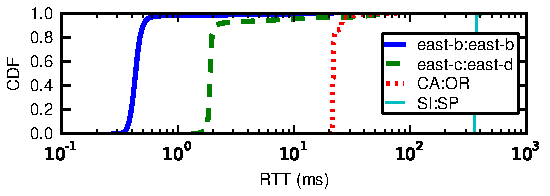
\includegraphics[width=\columnwidth]{graphs/ping-plot.pdf}
\caption{CDF of round-trip times for slowest inter- and intra-
  availability zone links compared to cross-region links.}
\label{fig:rtt}
\end{figure}

